%!TEX program = xelatex
\let\stop\empty

\documentclass[12pt,a4paper]{exam-zh}

\usepackage{xeCJK}
\setCJKmainfont{Noto Serif CJK SC}
\usepackage{geometry}
\usepackage{array}
\usepackage{tikz}
\usepackage{amsmath}
\usepackage{wrapfig}
\usepackage{adjustbox}
\usepackage{enumitem}
\usepackage{fancyhdr}
\usetikzlibrary{angles,quotes}

\usepackage{scalerel}
\def\mcirc{\mathbin{\scalerel*{\circ}{j}}}
\def\msquare{\mathord{\scalerel*{\Box}{gX}}}
\geometry{margin=2cm}

\AtBeginDocument{\zihao{4}}
% ----------- 调整 exam -----------


% --- 全局样式定义 ---
% 定义选择题环境：题号 1. 2.，选项 A. B. C. D. 粗体，且保留 1.5em 间距
\examsetup{
    page = {
    size = a4paper,           % 设定纸张大小 [4]
    foot-content = { - ; - }  % 页脚显示为 -1-, -2- 格式 [3]
  },
    choices = {
    label-pos = top-left,
    column-sep = 1em,
    label-pos = auto,
    label-sep = 0.5em,
    max-columns = 4
    },
  question = {
    top-sep    = 1em, % 调整题目上方的垂直距离（默认值为 .5em plus .5em minus .2em）
    bottom-sep = 1em  % 调整题目下方的垂直距离（默认值为 .5em plus .5em minus .2em）
  },
    paren = {
    show-paren = false  % 设置为 false 则不显示括号 [3, 4]
  },
    choices = {
    label = \textbf{\Alph*}
  }, 
    solution = {
    show-solution = show-move, % 答案自动移动到卷末
    label-content = {参考答案},  % 答案区的标题文字
    show-qed = true            % 在解答末尾显示结束符号 ◻ 
  }
}

% ==========================
% 卷面变量设置（只需改这里）
% ==========================
% ==========================
% 卷面变量设置（只需改这里）
% ==========================
\newcommand{\paperlevel}{高中一文商班}
\newcommand{\papersubject}{数学 试卷一}
\newcommand{\schoolname}{金宝培元独立中学}
\newcommand{\examname}{八月考}
\newcommand{\classinfo}{S1(Y / H)}
\newcommand{\examdate}{6-8-2026}
\newcommand{\examtime}{10:15-11:00}
\newcommand{\questiontotal}{16}
\newcommand{\paperpercentage}{40\%}
\newcommand{\setterteacher}{蔡杰庆师}
\newcommand{\reviewteacher}{王萌师}
\newcommand{\auditteacher}{雷泳健师}

\makeatletter
\newcounter{answerkeyquestion}
\let\answerkeytotal\questiontotal
\let\originalparen\paren
\newcommand{\answerkeyitems}{}
\newcommand{\addanswerkeyitem}[2]{%
  \pgfmathtruncatemacro{\row}{ifthenelse(#1<=\cols,0,1)}%
  \pgfmathtruncatemacro{\col}{mod(#1-1,\cols)}%
  \pgfmathsetlengthmacro{\x}{\col*\boxw}%
  \pgfmathsetlengthmacro{\y}{-\row*\boxh}%
  \draw (\x,\y) rectangle ++(\boxw,\boxh);%
  \node[anchor=north west] at (\x+\offset,\y+\boxh-\offset) {\textbf{#1.}};%
  \node at (\x+0.6*\boxw,\y+0.45*\boxh) {\Large\textbf{#2}};%
}
\renewcommand{\paren}[1][]{%
  \originalparen[#1]%
  \edef\answerkeytemp{#1}%
  \ifx\answerkeytemp\@empty\else
    \stepcounter{answerkeyquestion}%
    \begingroup
      \edef\x{\endgroup
        \noexpand\g@addto@macro\noexpand\answerkeyitems{\noexpand\addanswerkeyitem{\theanswerkeyquestion}{#1}}}%
    \x
  \fi
}
\makeatother

\begin{document}

% ==========================
% 三栏标题区
% ==========================
\noindent
\begin{tabular*}{\textwidth}{@{\extracolsep{\fill}} p{0.3\textwidth} p{0.35\textwidth} p{0.3\textwidth}}

\raggedright
\textbf{\paperlevel}\\[0.2em]
\textbf{}{\papersubject}\\[0.4em]
姓名：\underline{\hspace{3cm}} &

\centering
\textbf{\schoolname}\\[0.2em]
\textbf{\examname}\\[0.4em]
班级：\classinfo&

\raggedright
日期：\examdate\\[0.2em]
时间：\examtime\\[0.4em]
得分：\underline{\hspace{2.5cm}} \\

\end{tabular*}

\begin{flushleft}
考生须知： 
选出正确的答案，用蓝或黑色的原子笔将答案的相应选项字母填入本页特备作答栏。
\end{flushleft}

% =========================
% 答题栏
% =========================
\begin{flushleft}
\textbf{特备答题栏:}
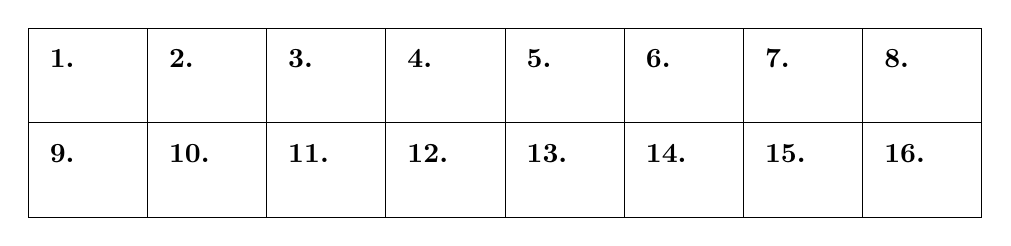
\begin{tikzpicture}
  % ---- 根据题数自动设置：16题为 8×2，20题为 10×2 ----
  \pgfmathtruncatemacro{\cols}{ifthenelse(\answerkeytotal<=16,8,10)}
  \pgfmathsetlengthmacro{\boxw}{(\linewidth-0.4pt)/\cols}
  \pgfmathsetlengthmacro{\boxh}{1.2cm}
  \pgfmathsetlengthmacro{\offset}{0.15cm}

  \foreach \num in {1,...,\answerkeytotal} {
    \pgfmathtruncatemacro{\row}{ifthenelse(\num<=\cols,0,1)}
    \pgfmathtruncatemacro{\col}{mod(\num-1,\cols)}
    \pgfmathsetlengthmacro{\x}{\col*\boxw}
    \pgfmathsetlengthmacro{\y}{-\row*\boxh}
    \draw (\x,\y) rectangle ++(\boxw,\boxh);
    \node[anchor=north west] at (\x+\offset,\y+\boxh-\offset) {\textbf{\num.}};
  }
\end{tikzpicture}

\end{flushleft}

\begin{question}
已知关于 $x$ 的不等式 $\dfrac{ax - 1}{x + 1} < 0$ 的解集为 $\{x \mid x < -1 \text{ 或 } x > -\dfrac{1}{2}\}$，则实数 $a$ 的值为： \paren[B]
    \begin{choices}
        \item $2$
        \item $-2$
        \item $\dfrac{1}{2}$
        \item $-\dfrac{1}{2}$
    \end{choices}
\end{question}
\begin{solution}
    \textbf{解析：}不等式 $\dfrac{ax - 1}{x + 1} < 0$ 的两个分界点分别为 $x=-1$ 和 $x=\dfrac{1}{a}$。

由已知解集为 $\{x \mid x < -1 \text{ 或 } x > -\frac{1}{2}\}$ 可知，另一个分界点为 $-\dfrac{1}{2}$，因此
\[
    \frac{1}{a}=-\frac{1}{2},
\]
解得
\[
    a=-2.
\]

检验：当 $a=-2$ 时，原不等式为
\[
    \frac{-2x-1}{x+1}<0,
\]
其解集为 $(-\infty,-1)\cup\left(-\frac{1}{2},+\infty\right)$，与题意相符。

故选 B。
\end{solution}

%region 范围：高中数学-分式不等式 | 考点：分式不等式的因式分解与符号分析法 | 难度：中等
\begin{question}
    解不等式 $\dfrac{2x^2-3x+1}{x^2+5x+6} \geq 0$ 。 \paren[A]
    \begin{choices}
        \item $x < -3$ 或 $-2 < x \leq \dfrac{1}{2}$ 或 $x \geq 1$
        \item $-3 < x < -2$ 或 $\dfrac{1}{2} < x < 1$
        \item $x \in \mathbb{R}$
        \item $x < -3$ 或 $-2 < x < \dfrac{1}{2}$ 或 $x > 1$
    \end{choices}
\end{question}

\begin{solution}
    求解不等式 $\dfrac{2x^2-3x+1}{x^2+5x+6} \geq 0$。 \\
    先将分子分母因式分解，再用符号分析法确定各区间正负。
    \begin{align*}
        \frac{2x^2-3x+1}{x^2+5x+6} &\geq 0 \\
        \frac{(2x-1)(x-1)}{(x+2)(x+3)} &\geq 0
    \end{align*}
    临界点为 $x=-3,-2,\dfrac{1}{2},1$，其中 $x=-3,-2$ 使分母为零（须排除），$x=\dfrac{1}{2},1$ 使分子为零（可取等）。列表判断各区间符号，得表达式在对应区间上非负。
    \[
        x < -3 \ \text{或} \ -2 < x \leq \frac{1}{2} \ \text{或} \ x \geq 1
    \]
    故选 A。
\end{solution}
%endregion


% \begin{question}已知关于 $x$ 的不等式 $ax^2+bx+c>0$ 的解集为 $(-1,2)$，则不等式 $cx^2-bx+a<0$ 的解集为： \paren[A]\begin{choices}
%     \item $\left(-\dfrac{1}{2},1\right)$
%     \item $\left(-\infty,-\dfrac{1}{2}\right)\cup(1,+\infty)$
%     \item $\left(-1,\dfrac{1}{2}\right)$
%     \item $(-\infty,-1)\cup\left(\dfrac{1}{2},+\infty\right)$
% \end{choices}
% \end{question}\begin{solution}\textbf{解析：}由不等式 $ax^2+bx+c>0$ 的解集为 $(-1,2)$ 可知：

% 1. $a<0$；
% 2. $x_1=-1$ 与 $x_2=2$ 是方程 $ax^2+bx+c=0$ 的两根。

% 由韦达定理得：
% \[
%     \begin{cases}
%         -1+2=-\dfrac{b}{a} \\
%         -1\times2=\dfrac{c}{a}
%     \end{cases}
%     \implies
%     \begin{cases}
%         b=-a \\
%         c=-2a
%     \end{cases}
% \]

% 将 $b,c$ 代入所求不等式 $cx^2-bx+a<0$：
% \[
%     -2ax^2+ax+a<0
% \]

% 因 $a<0$，两边同除以 $a$，不等号方向改变：
% \[
%     -2x^2+x+1>0
% \]
% 即：
% \[
%     2x^2-x-1<0
% \]

% 因式分解得：
% \[
%     (2x+1)(x-1)<0
% \]

% 解得 $-\dfrac{1}{2}<x<1$。

% 故选 A。
% \end{solution}

%region 范围：不等式 | 考点：分式不等式的解法与等价转化 | 难度：中等
\begin{question}
    已知实数 $x$ 满足分式不等式 $\displaystyle\frac{2x-1}{x+1} \ge 1$，则该不等式的解集为 \paren[C]
    \begin{choices}
        \item $\{x \mid x \ge 2\}$
        \item $\{x \mid x > -1\}$
        \item $\{x \mid x \ge 2 \text{ 或 } x < -1\}$
        \item $\{x \mid -1 < x \le 2\}$
    \end{choices}
\end{question}

\begin{solution}
    \textbf{解析：} \\
    首先分析题意，原不等式为分式不等式，不能直接去分母（因为分母 $x+1$ 的正负号不确定）。我们需要通过移项、通分，将其转化为标准形式。 \\
    将不等式右边的 $1$ 移到左边，得：
    \[ \displaystyle\frac{2x-1}{x+1} - 1 \ge 0 \]
    进行通分化简：
    \[ \displaystyle\frac{(2x-1) - (x+1)}{x+1} \ge 0 \]
    \[ \displaystyle\frac{x-2}{x+1} \ge 0 \]
    根据分式不等式的等价转化原理，上述不等式等价于整式不等式组：
    \[ \displaystyle \begin{cases} (x-2)(x+1) \ge 0 \\ x+1 \neq 0 \end{cases} \]
    解这个不等式组，由 $(x-2)(x+1) \ge 0$ 可得 $x \ge 2$ 或 $x \le -1$。 \\
    又因为分母不能为零，即 $x \neq -1$，所以最终的解集为 $\{x \mid x \ge 2 \text{ 或 } x < -1\}$。 \\
    
    \textbf{干扰项分析：} \\
    * 选项 A：忽略了分母为负数时的情况，直接视同 $2x-1 \ge x+1$ 去分母导致漏解。 \\
    * 选项 B：对不等号方向或因式分解边界点判断错误。 \\
    * 选项 D：将不等式的解集区间方向弄反（错解为 $-1 < x \le 2$），属于典型的“大于取两边，小于取中间”概念混淆。 \\
    故选 C。
\end{solution}
%endregion

%region 范围：函数 | 考点：函数的定义与垂直线检验法（Vertical Line Test） | 难度：中等
\begin{question}
    在平面直角坐标系 $xOy$ 中，下列各图所示的曲线中，能表示 $y$ 是 $x$ 的函数的是 \paren[B]
    \begin{choices}
        \item 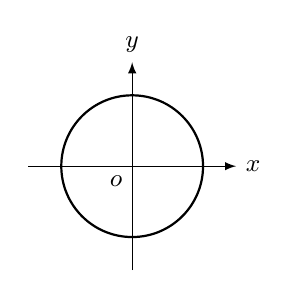
\begin{tikzpicture}[scale=0.6, baseline=(current bounding box.center)]
                \draw[-latex] (-2.2,0) -- (2.2,0) node[right] {\small $x$};
                \draw[-latex] (0,-2.2) -- (0,2.2) node[above] {\small $y$};
                \node[below left] at (0,0) {\small $o$};
                \draw[thick] (0,0) circle (1.5);
              \end{tikzpicture}
        \item 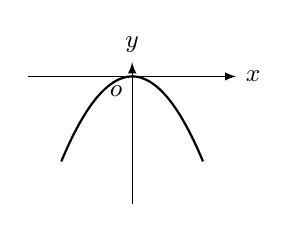
\begin{tikzpicture}[scale=0.6, baseline=(current bounding box.center)]
                \draw[-latex] (-2.2,2.2) -- (2.2,2.2) node[right] {\small $x$}; % 调整坐标轴位置适配抛物线
                \draw[-latex] (0,-0.5) -- (0,2.5) node[above] {\small $y$};
                \node[below left] at (0,2.2) {\small $o$};
                \draw[thick, domain=-1.5:1.5, samples=50, smooth] plot (\x, {2.2 - 0.8*\x*\x});
              \end{tikzpicture}
        \item \begin{tikzpicture}[scale=0.6, baseline=(current bounding box.center)]
                \draw[-latex] (-1,0) -- (2.5,0) node[right] {\small $x$};
                \draw[-latex] (0,-1.8) -- (0,1.8) node[above] {\small $y$};
                \node[below left] at (0,0) {\small $o$};
                \draw[thick, domain=-1.3:1.3, samples=50, smooth] plot ({1.2 + 0.5*\x*\x}, \x);
              \end{tikzpicture}
        \item 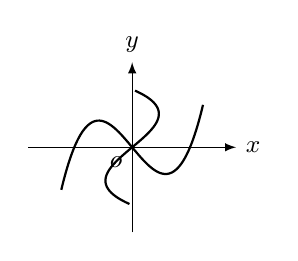
\begin{tikzpicture}[scale=0.6, baseline=(current bounding box.center)]
                \draw[-latex] (-2.2,0) -- (2.2,0) node[right] {\small $x$};
                \draw[-latex] (0,-1.8) -- (0,1.8) node[above] {\small $y$};
                \node[below left] at (0,0) {\small $o$};
                \draw[thick, domain=-1.5:1.5, samples=60, smooth] plot (\x, {0.8*\x*\x*\x - 1.2*\x});
                % 旋转或修改使其不满足函数定义（令其多值）
                \begin{scope}[rotate=90]
                \draw[thick, domain=-1.2:1.2, samples=60, smooth] plot (\x, {0.8*\x*\x*\x - 1.2*\x});
                \end{scope}
              \end{tikzpicture}
    \end{choices}
\end{question}

\begin{solution}
    \textbf{解析：} \\
    首先分析题意，本题考查的是函数的定义及其几何意义。根据函数的定义：设 $A, B$ 是两个非空的数集，如果按照某种确定的对应关系 $f$，使对于集合 $A$ 中的任意一个数 $x$，在集合 $B$ 中都有唯一确定的数 $y$ 和它对应，那么就称 $y$ 是 $x$ 的函数。 \\
    在几何图像上的表现即为**垂直线检验法（Vertical Line Test）**：作一条垂直于 $x$ 轴的直线 $x = a$，若该直线与曲线最多只有一个交点，则表示 $y$ 是 $x$ 的函数；若存在交点多于一个的情况，则说明一个 $x$ 对应了多个 $y$，不符合函数的唯一性要求。 \\
    
    下面逐一检验各选项： \\
    * 选项 A：该图像是一个圆。作一条通过圆心的垂直于 $x$ 轴的直线，显而易见该直线与圆有两个交点（即一个 $x$ 对应了两个不同的 $y$ 值），故不能表示 $y$ 是 $x$ 的函数。 \\
    * 选项 B：该图像是一条开口向下的抛物线。任意作一条垂直于 $x$ 轴的直线，与该抛物线至多只有一个交点，满足对于每一个任意的 $x$，都有唯一确定的 $y$ 与之对应，故能表示 $y$ 是 $x$ 的函数。 \\
    * 选项 C：该图像是开口向右的抛物线。作直线 $x = 1.5$，该直线与曲线有两个交点，不满足唯一性，故不能表示 $y$ 是 $x$ 的函数。 \\
    * 选项 D：该曲线呈现“S”型或交叉的多值曲线。作一条垂直于 $x$ 轴的直线穿过其弯曲或重叠部分，显然可以与曲线产生三个交点，即一个 $x$ 对应了三个 $y$ 值，不符合函数定义。 \\
    故选 B。
\end{solution}
%endregion

%region 范围：函数 | 考点：函数的概念与韦恩图（Venn diagram）表示法 | 难度：中等
\begin{question}
    设集合 $A = \{1, 2, 3\}$，集合 $B = \{a, b, c\}$，下列各范恩图（Venn）所示的对应关系 $f$ 中，能构成从集合 $A$ 到集合 $B$ 的函数的是 \paren[D]
    \begin{choices}
        \item 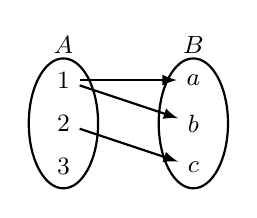
\begin{tikzpicture}[scale=0.55, baseline=(current bounding box.center)]
                % 集合 A
                \draw[thick] (0,0) ellipse (0.8cm and 1.5cm);
                \node at (0,1.8) {\small $A$};
                \node (A1) at (0,1) {\small 1};
                \node (A2) at (0,0) {\small 2};
                \node (A3) at (0,-1) {\small 3};
                % 集合 B
                \draw[thick] (3,0) ellipse (0.8cm and 1.5cm);
                \node at (3,1.8) {\small $B$};
                \node (B1) at (3,1) {\small $a$};
                \node (B2) at (3,0) {\small $b$};
                \node (B3) at (3,-1) {\small $c$};
                % 映射箭头
                \draw[-latex, thick] (A1) -- (B1);
                \draw[-latex, thick] (A1) -- (B2);
                \draw[-latex, thick] (A2) -- (B3);
              \end{tikzpicture}
        \item 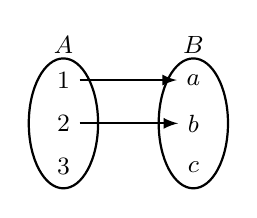
\begin{tikzpicture}[scale=0.55, baseline=(current bounding box.center)]
                % 集合 A
                \draw[thick] (0,0) ellipse (0.8cm and 1.5cm);
                \node at (0,1.8) {\small $A$};
                \node (A1) at (0,1) {\small 1};
                \node (A2) at (0,0) {\small 2};
                \node (A3) at (0,-1) {\small 3};
                % 集合 B
                \draw[thick] (3,0) ellipse (0.8cm and 1.5cm);
                \node at (3,1.8) {\small $B$};
                \node (B1) at (3,1) {\small $a$};
                \node (B2) at (3,0) {\small $b$};
                \node (B3) at (3,-1) {\small $c$};
                % 映射箭头
                \draw[-latex, thick] (A1) -- (B1);
                \draw[-latex, thick] (A2) -- (B2);
              \end{tikzpicture}
        \item 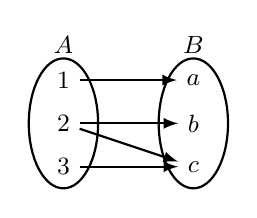
\begin{tikzpicture}[scale=0.55, baseline=(current bounding box.center)]
                % 集合 A
                \draw[thick] (0,0) ellipse (0.8cm and 1.5cm);
                \node at (0,1.8) {\small $A$};
                \node (A1) at (0,1) {\small 1};
                \node (A2) at (0,0) {\small 2};
                \node (A3) at (0,-1) {\small 3};
                % 集合 B
                \draw[thick] (3,0) ellipse (0.8cm and 1.5cm);
                \node at (3,1.8) {\small $B$};
                \node (B1) at (3,1) {\small $a$};
                \node (B2) at (3,0) {\small $b$};
                \node (B3) at (3,-1) {\small $c$};
                % 映射箭头
                \draw[-latex, thick] (A1) -- (B1);
                \draw[-latex, thick] (A2) -- (B2);
                \draw[-latex, thick] (A2) -- (B3);
                \draw[-latex, thick] (A3) -- (B3);
              \end{tikzpicture}
        \item 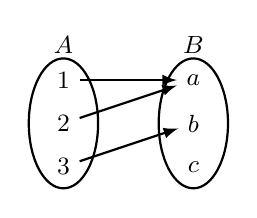
\begin{tikzpicture}[scale=0.55, baseline=(current bounding box.center)]
                % 集合 A
                \draw[thick] (0,0) ellipse (0.8cm and 1.5cm);
                \node at (0,1.8) {\small $A$};
                \node (A1) at (0,1) {\small 1};
                \node (A2) at (0,0) {\small 2};
                \node (A3) at (0,-1) {\small 3};
                % 集合 B
                \draw[thick] (3,0) ellipse (0.8cm and 1.5cm);
                \node at (3,1.8) {\small $B$};
                \node (B1) at (3,1) {\small $a$};
                \node (B2) at (3,0) {\small $b$};
                \node (B3) at (3,-1) {\small $c$};
                % 映射箭头
                \draw[-latex, thick] (A1) -- (B1);
                \draw[-latex, thick] (A2) -- (B1);
                \draw[-latex, thick] (A3) -- (B2);
              \end{tikzpicture}
    \end{choices}
\end{question}

\begin{solution}
    \textbf{解析：} \\
    首先分析题意，本题通过韦恩图考查函数的定义。函数的定义包含两个核心要点：
    \begin{enumerate}
        \item \textbf{定义域的任意性}：定义域（集合 $A$）中的**每一个**元素都必须在到达域（集合 $B$）中有对应。即集合 $A$ 中不能有“漏掉”的元素（每个元素都要有箭头射出）。
        \item \textbf{对应关系的唯一性}：集合 $A$ 中的任意一个元素，在集合 $B$ 中有且只有**唯一**的一个元素与之对应。即集合 $A$ 中的每个元素只能射出一条箭头（不能“一射多”，但允许“多射一”，且集合 $B$ 中允许有剩余元素）。
    \end{enumerate}
    
    下面对各选项进行逐一分析： \\
    * 选项 A：元素 $1$ 对应了 $a$ 和 $b$ 两个元素（一射多），不满足唯一性；同时元素 $3$ 没有对应元素，不满足任意性，故不是函数。 \\
    * 选项 B：元素 $3$ 没有对应元素，导致集合 $A$ 中的元素没有全部被使用，不满足任意性，故不是函数。 \\
    * 选项 C：元素 $2$ 同时对应了 $b$ 和 $c$ 两个元素（一射多），不满足唯一性，故不是函数。 \\
    * 选项 D：集合 $A$ 中的每个元素都有箭头射出（满足任意性），且每个元素都只射出了一条箭头（满足唯一性，虽然 $1$ 和 $2$ 同时指向了 $a$，但对 $1$ 和 $2$ 自身而言，其对应值都是唯一的），完全符合函数的定义。 \\
    故选 D。
\end{solution}
%endregion

% %region 范围：函数 | 考点：分式、一元二次方程判别式法 | 难度：难
% \begin{question}
%     求函数 $\displaystyle f(x) = \frac{x^2 - x + 1}{x^2 + x + 1}$ 的值域。\paren[A]
%     \begin{choices}
%         \item $\displaystyle \left[ \frac{1}{3}, 3 \right]$
%         \item $\displaystyle \left( \frac{1}{3}, 3 \right)$
%         \item $\displaystyle \left( -\infty, \frac{1}{3} \right] \cup [3, +\infty)$
%         \item $\displaystyle \left[ -3, -\frac{1}{3} \right]$
%     \end{choices}
% \end{question}

% \begin{solution}
%     \textbf{解析：} \\
%     步骤 1：分析题意与知识点引入。\\
%     本题要求分式函数的值域。由于分子分母均为一元二次多项式，且定义域为 $x \in \mathbb{R}$（因为分母 $x^2 + x + 1 = (x + \frac{1}{2})^2 + \frac{3}{4} > 0$ 恒成立），最常用的解题策略是“反求法”或“一元二次方程判别式法”。令 $\displaystyle y = \frac{x^2 - x + 1}{x^2 + x + 1}$，将其转化为关于 $x$ 的一元二次方程。\\

%     步骤 2：公式计算与推导验证。\\
%     去分母并整理，可得：
%     \[ \displaystyle y(x^2 + x + 1) = x^2 - x + 1 \]
%     \[ \displaystyle (y - 1)x^2 + (y + 1)x + (y - 1) = 0 \]
    
%     分类讨论：
%     当 $y = 1$ 时，方程化为 $2x = 0$，解得 $x = 0$。即 $x=0$ 时，$y=1$，所以 $1$ 在值域内。
    
%     当 $y \neq 1$ 时，上述方程为关于 $x$ 的一元二次方程。由于 $x \in \mathbb{R}$，方程必须有实数根，故判别式 $\Delta \ge 0$。
%     \[ \displaystyle \Delta = (y + 1)^2 - 4(y - 1)^2 \ge 0 \]
%     展开并化简：
%     \[ \displaystyle y^2 + 2y + 1 - 4(y^2 - 2y + 1) \ge 0 \]
%     \[ \displaystyle -3y^2 + 10y - 3 \ge 0 \]
%     两边同乘 $-1$ 改变不等号方向：
%     \[ \displaystyle 3y^2 - 10y + 3 \le 0 \]
%     十字相乘因式分解：
%     \[ \displaystyle (3y - 1)(y - 3) \le 0 \]
%     解得：$\displaystyle \frac{1}{3} \le y \le 3$。
%     又因为当 $y=1$ 时也在此区间内，故所求值域为 $\displaystyle \left[ \frac{1}{3}, 3 \right]$。\\
    
%     以下为该函数的图像辅助理解，可明显看出其上下界：
%     \begin{center}
%     \begin{tikzpicture}[scale=1.2]
%         % 坐标轴
%         \draw[->] (-4,0) -- (4,0) node[right] {$x$};
%         \draw[->] (0,-0.5) -- (0,3.5) node[above] {$y$};
%         \node[below left] at (0,0) {$O$};
        
%         % 绘制函数曲线
%         \draw[smooth, samples=100, domain=-3.5:3.5, thick, blue] plot (\x, {(\x*\x - \x + 1)/(\x*\x + \x + 1)});
        
%         % 辅助线：最大值与最小值
%         \draw[dashed, red] (-4,3) -- (4,3) node[right] {$y=3$};
%         \draw[dashed, red] (-4,0.333) -- (4,0.333) node[right] {$y=\frac{1}{3}$};
        
%         % 极值点标注
%         \filldraw[black] (-1,3) circle (1.5pt) node[above left] {$(-1, 3)$};
%         \filldraw[black] (1,0.333) circle (1.5pt) node[below right] {$(1, \frac{1}{3})$};
%     \end{tikzpicture}
%     \end{center}
    
%     步骤 3：结论梳理与干扰项分析。\\
%     正确答案为 $\displaystyle \left[ \frac{1}{3}, 3 \right]$。\\
%     干扰项 B 错误，因为学生在求解 $\Delta \ge 0$ 时可能误写为严格大于号 $\Delta > 0$，忽略了等号（即函数能取到最值）；\\
%     干扰项 C 错误，这是解不等式 $-3y^2 + 10y - 3 \ge 0$ 时，未变号直接求两边区间导致的典型错误；\\
%     干扰项 D 错误，这是在分解因式 $(3y - 1)(y - 3)$ 时发生正负号混淆所致。\\
    
%     故选 A。
% \end{solution}
% %endregion


%region 范围：高中数学 - 函数 | 考点：分段函数逆向求值（已知函数值求自变量） | 难度：中等
\begin{question}
    设函数 $f(x)$ 定义为三段分段函数，其表达式为：
    $$f(x) = \begin{cases} x + 3, & x < 0 \\ x^2 - 1, & 0 \leq x < 2 \\ 2x - 1, & x \geq 2 \end{cases}$$
    若 $f(a) = 3$，求 $a$ 的值。 \paren[B]
    \begin{choices}
        \item $a = 0$
        \item $a = 2$
        \item $a = -2$
        \item $a = 4$
    \end{choices}
\end{question}

\begin{solution}
    \textbf{解析：} \\
    本题的关键在于：由于 $f(x)$ 为分段函数，求解 $f(a) = 3$ 时必须**逐段假设并代入**，
    再检验所得的 $a$ 值是否真正落在该段所对应的定义区间内，唯有区间条件成立的解才是合理解。 \\[4pt]
    \textbf{第一段（$x < 0$）：} 假设 $a$ 落在此区间，代入 $f(x) = x + 3$：
    \[ \displaystyle a + 3 = 3 \implies a = 0 \]
    但 $a = 0$ 并不满足 $x < 0$ 的条件，故此段无解（选项 A 即为忽略区间检验而误取此值所致）。 \\[4pt]
    \textbf{第二段（$0 \leq x < 2$）：} 假设 $a$ 落在此区间，代入 $f(x) = x^2 - 1$：
    \[ \displaystyle a^2 - 1 = 3 \implies a^2 = 4 \implies a = 2 \text{ 或 } a = -2 \]
    检验区间 $0 \leq x < 2$：$a = 2$ 不满足（因 $2$ 不小于 $2$），$a = -2$ 也不满足（为负值）。
    故此段两个根均须舍去（选项 C 即为只取负根却未检验区间范围所致的错误）。 \\[4pt]
    \textbf{第三段（$x \geq 2$）：} 假设 $a$ 落在此区间，代入 $f(x) = 2x - 1$：
    \[ \displaystyle 2a - 1 = 3 \implies 2a = 4 \implies a = 2 \]
    检验：$a = 2$ 满足 $x \geq 2$ 的条件，故此解成立。 \\
    （选项 D 中的 $a = 4$ 属于移项后误将 $2a = 4$ 直接当作最终答案，遗漏了两边除以 $2$ 的步骤所致的计算错误）。 \\[4pt]
    综上，唯一合理解为 $a = 2$，故选 B。
\end{solution}
%endregion

%region 范围：高中数学 - 函数的复合与待定系数法 | 考点：函数复合（f(f(x))）、待定系数法解方程组 | 难度：中等
\begin{question}
    已知函数 $f(x) = mx + n$（其中 $m, n$ 均为常数，且 $m > 0$），对任意实数 $x$ 恒有$f(f(x)) = 4x + 9$，求 $f(x)$ 。 \paren[C]
    \begin{choices}
        \item $f(x) = -2x - 9$
        \item $f(x) = 2x - 3$
        \item $f(x) = 2x + 3$
        \item $f(x) = 4x + 3$
    \end{choices}
\end{question}

\begin{solution}
    \textbf{解析：} \\
    设 $f(x) = mx + n$，代入复合函数 $f(f(x))$ 的定义，得：
    \[ \displaystyle f(f(x)) = m(mx + n) + n = m^2 x + (mn + n) \]
    将其与已知条件 $f(f(x)) = 4x + 9$ 逐项比较系数（一次项系数相等，常数项也相等），可得方程组：
    \[ \displaystyle m^2 = 4, \qquad n(m + 1) = 9 \]
    由 $m^2 = 4$ 解得 $m = 2$ 或 $m = -2$。 \\
    但题目已限定 $m > 0$，故舍去 $m = -2$ 这一情形 \\
    （选项 A 的 $f(x) = -2x - 9$ 恰好对应 $m = -2$ 时的解：此时 $n(-2+1) = 9 \implies n = -9$，
    虽然代数上同样满足 $f(f(x)) = 4x + 9$，但违反了题目 $m > 0$ 的限定条件，应予排除）。 \\[4pt]
    取 $m = 2$，代入 $n(m+1) = 9$：
    \[ \displaystyle n(2 + 1) = 9 \implies 3n = 9 \implies n = 3 \]
    故 $f(x) = 2x + 3$。 \\[4pt]
    验证：$f(f(x)) = 2(2x+3) + 3 = 4x + 6 + 3 = 4x + 9$，与题设吻合，成立。 \\[4pt]
    对于选项 B（$f(x) = 2x - 3$），属于符号错误：将 $n(m+1)=9$ 误解为 $n(m-1)=9$，
    从而错误地得到 $n = -3$。 \\
    对于选项 D（$f(x) = 4x + 3$），属于系数混淆错误：将 $m^2 = 4$ 误当作 $m = 4$ 直接代入，
    而未对 $m^2$ 正确开方求解。 \\[4pt]
    综上，唯一满足 $m > 0$ 且符合题设的解为 $f(x) = 2x + 3$，故选 C。
\end{solution}
%endregion

%region 范围：高中数学 - 二次函数的图象与性质 | 考点：抛物线开口方向、顶点、与坐标轴交点的图象判断 | 难度：中等
\begin{question}
    已知二次函数 $y = x^2 -2x -3 $,
    下列哪一个图象正确地表示了该函数？ \paren[A]
    \begin{choices}
        \item
        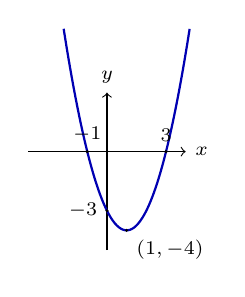
\begin{tikzpicture}[scale=0.25, baseline={(0,0)}]
            \draw[->] (-4,0) -- (4,0) node[right] {\scriptsize $x$};
            \draw[->] (0,-5) -- (0,3) node[above] {\scriptsize $y$};
            \draw[thick, blue!70!black, domain=-2.2:4.2, samples=60, smooth]
                plot (\x, {(\x)^2 - 2*\x - 3});
            \filldraw (1,-4) circle (1.3pt) node[below right, font=\scriptsize] {$(1,-4)$};
            \filldraw (-1,0) circle (1.3pt) node[above, font=\scriptsize] {$-1$};
            \filldraw (3,0) circle (1.3pt) node[above, font=\scriptsize] {$3$};
            \filldraw (0,-3) circle (1.3pt) node[left, font=\scriptsize] {$-3$};
        \end{tikzpicture}

        \item
        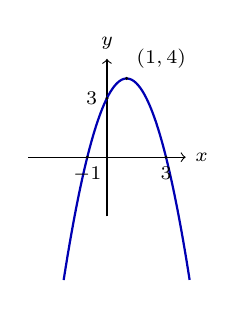
\begin{tikzpicture}[scale=0.25, baseline={(0,0)}]
            \draw[->] (-4,0) -- (4,0) node[right] {\scriptsize $x$};
            \draw[->] (0,-3) -- (0,5) node[above] {\scriptsize $y$};
            \draw[thick, blue!70!black, domain=-2.2:4.2, samples=60, smooth]
                plot (\x, {-((\x)^2 - 2*\x - 3)});
            \filldraw (1,4) circle (1.3pt) node[above right, font=\scriptsize] {$(1,4)$};
            \filldraw (-1,0) circle (1.3pt) node[below, font=\scriptsize] {$-1$};
            \filldraw (3,0) circle (1.3pt) node[below, font=\scriptsize] {$3$};
            \filldraw (0,3) circle (1.3pt) node[left, font=\scriptsize] {$3$};
        \end{tikzpicture}

        \item
        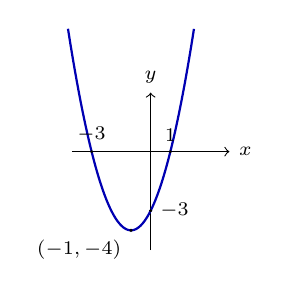
\begin{tikzpicture}[scale=0.25, baseline={(0,0)}]
            \draw[->] (-4,0) -- (4,0) node[right] {\scriptsize $x$};
            \draw[->] (0,-5) -- (0,3) node[above] {\scriptsize $y$};
            \draw[thick, blue!70!black, domain=-4.2:2.2, samples=60, smooth]
                plot (\x, {(\x)^2 + 2*\x - 3});
            \filldraw (-1,-4) circle (1.3pt) node[below left, font=\scriptsize] {$(-1,-4)$};
            \filldraw (-3,0) circle (1.3pt) node[above, font=\scriptsize] {$-3$};
            \filldraw (1,0) circle (1.3pt) node[above, font=\scriptsize] {$1$};
            \filldraw (0,-3) circle (1.3pt) node[right, font=\scriptsize] {$-3$};
        \end{tikzpicture}

        \item
        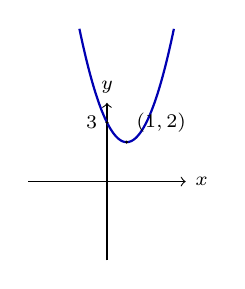
\begin{tikzpicture}[scale=0.25, baseline={(0,0)}]
            \draw[->] (-4,0) -- (4,0) node[right] {\scriptsize $x$};
            \draw[->] (0,-4) -- (0,4) node[above] {\scriptsize $y$};
            \draw[thick, blue!70!black, domain=-1.4:3.4, samples=60, smooth]
                plot (\x, {(\x)^2 - 2*\x + 3});
            \filldraw (1,2) circle (1.3pt) node[above right, font=\scriptsize] {$(1,2)$};
            \filldraw (0,3) circle (1.3pt) node[left, font=\scriptsize] {$3$};
        \end{tikzpicture}
    \end{choices}
\end{question}

\begin{solution}
    \textbf{解析：} \\
    已知 $a = 1 > 0$，$b = -2$，$c = -3$，代入函数得 $y = x^2 - 2x - 3$。 \\[4pt]
    \textbf{开口方向：} 由 $a = 1 > 0$ 可知，抛物线开口向上。
    选项 B 的图象开口向下，对应的是 $a = -1$ 的情形（即整体取相反数），与题设 $a=1$ 不符，应排除。 \\[4pt]
    \textbf{顶点坐标：} 顶点横坐标为
    \[ \displaystyle x_0 = -\frac{b}{2a} = -\frac{-2}{2(1)} = 1 \]
    代入原函数求纵坐标：
    \[ \displaystyle y_0 = (1)^2 - 2(1) - 3 = 1 - 2 - 3 = -4 \]
    故顶点为 $(1, -4)$。 \\
    选项 C 的顶点为 $(-1, -4)$，其错误在于顶点公式中把 $-\frac{b}{2a}$ 的符号算反
    （误用 $x_0 = \frac{b}{2a} = \frac{-2}{2} = -1$），应排除。 \\[4pt]
    \textbf{与坐标轴的交点：} 令 $y=0$，即 $x^2-2x-3=0$，分解得 $(x-3)(x+1)=0$，
    故与 $x$ 轴交于 $(-1,0)$ 和 $(3,0)$；令 $x=0$，得 $y=c=-3$，即与 $y$ 轴交于 $(0,-3)$。 \\
    选项 D 的图象与 $y$ 轴交于 $(0,3)$（正值），其错误在于将常数项 $c=-3$ 的符号弄反直接代入，
    导致整条图象在纵向发生错误平移，且此图象与 $x$ 轴无交点，与本题判别式
    $\Delta = b^2-4ac = 4+12=16>0$（应有两个不同实根）的结论矛盾，应排除。 \\[4pt]
    综上，唯一同时满足开口向上、顶点为 $(1,-4)$、与坐标轴正确相交的图象为选项 A，故选 A。
\end{solution}
%endregion


%region 范围：高中数学 - 反函数 | 考点：反函数的图象与原函数图象关于直线 y=x 对称 | 难度：中等
    \begin{question}
        已知函数 $y = (x-1)^2$，其定义域 $D_f = [1, +\infty)$，图象如图所示：

        \begin{center}
        \begin{tikzpicture}[scale=0.7]
            \draw[->] (-1,0) -- (4.5,0) node[right] {\scriptsize $x$};
            \draw[->] (0,-1) -- (0,4.5) node[above] {\scriptsize $y$};
            \node[below left] at (0,0) {\scriptsize $O$};
            \draw[thick, blue!70!black, domain=1:3, samples=60, smooth]
                plot (\x, {(\x-1)^2});
            \filldraw (1,0) circle (1.5pt) node[below, font=\scriptsize] {$(1,0)$};
            \filldraw (2,1) circle (1.5pt) node[right, font=\scriptsize] {$(2,1)$};
            \filldraw (3,4) circle (1.5pt) node[above, font=\scriptsize] {$(3,4)$};
        \end{tikzpicture}
        \end{center}

        下列哪一个图象是其反函数的图象？ \paren[B]
        \begin{choices}
            \item
            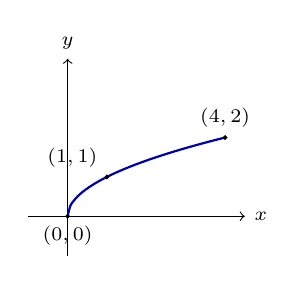
\begin{tikzpicture}[scale=0.5, baseline={(0,0)}]
                \draw[->] (-1,0) -- (4.5,0) node[right] {\scriptsize $x$};
                \draw[->] (0,-1) -- (0,4) node[above] {\scriptsize $y$};
                \draw[thick, blue!70!black, domain=0:4, samples=60, smooth]
                    plot (\x, {sqrt(\x)});
                \filldraw (0,0) circle (1.3pt) node[below, font=\scriptsize] {$(0,0)$};
                \filldraw (1,1) circle (1.3pt) node[above left, font=\scriptsize] {$(1,1)$};
                \filldraw (4,2) circle (1.3pt) node[above, font=\scriptsize] {$(4,2)$};
            \end{tikzpicture}

            \item
            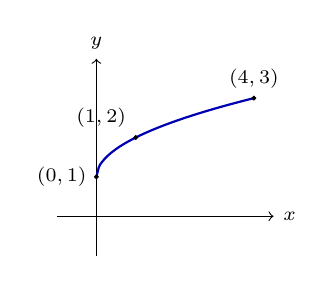
\begin{tikzpicture}[scale=0.5, baseline={(0,0)}]
                \draw[->] (-1,0) -- (4.5,0) node[right] {\scriptsize $x$};
                \draw[->] (0,-1) -- (0,4) node[above] {\scriptsize $y$};
                \draw[thick, blue!70!black, domain=0:4, samples=60, smooth]
                    plot (\x, {1+sqrt(\x)});
                \filldraw (0,1) circle (1.3pt) node[left, font=\scriptsize] {$(0,1)$};
                \filldraw (1,2) circle (1.3pt) node[above left, font=\scriptsize] {$(1,2)$};
                \filldraw (4,3) circle (1.3pt) node[above, font=\scriptsize] {$(4,3)$};
            \end{tikzpicture}

            \item
            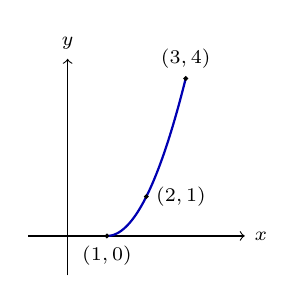
\begin{tikzpicture}[scale=0.5, baseline={(0,0)}]
                \draw[->] (-1,0) -- (4.5,0) node[right] {\scriptsize $x$};
                \draw[->] (0,-1) -- (0,4.5) node[above] {\scriptsize $y$};
                \draw[thick, blue!70!black, domain=1:3, samples=60, smooth]
                    plot (\x, {(\x-1)^2});
                \filldraw (1,0) circle (1.3pt) node[below, font=\scriptsize] {$(1,0)$};
                \filldraw (2,1) circle (1.3pt) node[right, font=\scriptsize] {$(2,1)$};
                \filldraw (3,4) circle (1.3pt) node[above, font=\scriptsize] {$(3,4)$};
            \end{tikzpicture}

            \item
            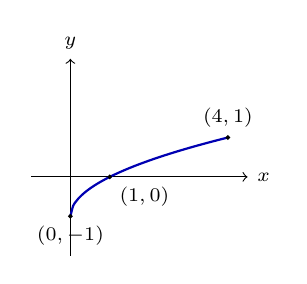
\begin{tikzpicture}[scale=0.5, baseline={(0,0)}]
                \draw[->] (-1,0) -- (4.5,0) node[right] {\scriptsize $x$};
                \draw[->] (0,-2) -- (0,3) node[above] {\scriptsize $y$};
                \draw[thick, blue!70!black, domain=0:4, samples=60, smooth]
                    plot (\x, {-1+sqrt(\x)});
                \filldraw (0,-1) circle (1.3pt) node[below, font=\scriptsize] {$(0,-1)$};
                \filldraw (1,0) circle (1.3pt) node[below right, font=\scriptsize] {$(1,0)$};
                \filldraw (4,1) circle (1.3pt) node[above, font=\scriptsize] {$(4,1)$};
            \end{tikzpicture}
        \end{choices}
    \end{question}

\begin{solution}
    \textbf{解析：} \\
    求反函数的核心方法是：将原函数 $y = (x-1)^2$（$D_f = [1, +\infty)$）中的 $x$、$y$ 互换角色后重新解出 $y$，
    再对照原函数的值域（即反函数的定义域）确定取舍。 \\[4pt]
    \textbf{第一步：交换变量。} \\
    将 $x$ 与 $y$ 互换，得：
    \[ \displaystyle x = (y-1)^2 \]
    \textbf{第二步：解出 $y$。} \\
    两边开方：
    \[ \displaystyle y - 1 = \pm\sqrt{x} \]
    由于原函数定义域为 $D_f = [1, +\infty)$，其值域为 $y \geq 0$；反函数的值域应等于原函数的定义域，
    即反函数的 $y \geq 1$，故此处只能取正号：
    \[ \displaystyle y = 1 + \sqrt{x} \]
    \textbf{第三步：确定反函数定义域。} \\
    原函数的值域 $y \geq 0$ 即为反函数的定义域，故反函数为 $y = 1 + \sqrt{x}$，其定义域为 $[0, +\infty)$。 \\[4pt]
    \textbf{验证关键点：} 原函数上的点 $(1,0)$、$(2,1)$、$(3,4)$ 关于直线 $y=x$ 对称后，
    应分别对应反函数上的点 $(0,1)$、$(1,2)$、$(4,3)$，这与选项 B 完全吻合。 \\[4pt]
    对于选项 A（$y=\sqrt{x}$），其错误在于求解过程中遗漏了常数项 $+1$，
    误将 $y-1=\sqrt{x}$ 直接当作 $y=\sqrt{x}$，导致整条曲线沿纵向少平移了 $1$ 个单位。 \\
    对于选项 C，该图象与原函数图象完全相同，属于误以为"原函数与反函数图象一致"，
    未对变量进行互换、也未关于直线 $y=x$ 作对称变换所致的错误。 \\
    对于选项 D（$y=-1+\sqrt{x}$），其错误在于符号处理有误，
    将 $y-1=\sqrt{x}$ 中的 $-1$ 误移项为 $y=\sqrt{x}-1$（等价于把常数项符号弄反）。 \\[4pt]
    综上，唯一正确表示反函数图象（即与原图象关于直线 $y=x$ 对称）的选项为 B，故选 B。
\end{solution}
%endregion

\newpage

%region 范围：高中数学 - 二元一次不等式组表示的平面区域 | 考点：不等式组的整理（移项、变号）与区域图象判断 | 难度：困难
\begin{question}
    在平面直角坐标系中，下列不等式组所表示的平面区域（阴影部分）是哪一个图象？
    $$\begin{cases} 4 \geq x + y \\ y - x \geq -2 \\ x + 1 \geq 0 \end{cases}$$
    \paren[A]
    \begin{choices}
        \item
        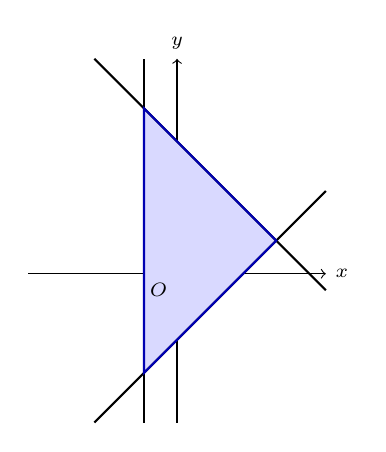
\begin{tikzpicture}[scale=0.42, baseline={(0,1)}]
            \draw[->] (-4.5,0) -- (4.5,0) node[right] {\scriptsize $x$};
            \draw[->] (0,-4.5) -- (0,6.5) node[above] {\scriptsize $y$};
            \fill[blue!15] (-1,-3) -- (3,1) -- (-1,5) -- cycle;
            \draw[thick] (-2.5,6.5) -- (4.5,-0.5); % 直线 x+y=4
            \draw[thick] (-2.5,-4.5) -- (4.5,2.5); % 直线 y-x=-2
            \draw[thick] (-1,-4.5) -- (-1,6.5);    % 直线 x=-1
            \draw[thick, blue!70!black] (-1,-3) -- (3,1) -- (-1,5) -- cycle;
            \node[below left] at (0,0) {\scriptsize $O$};
        \end{tikzpicture}

        \item
        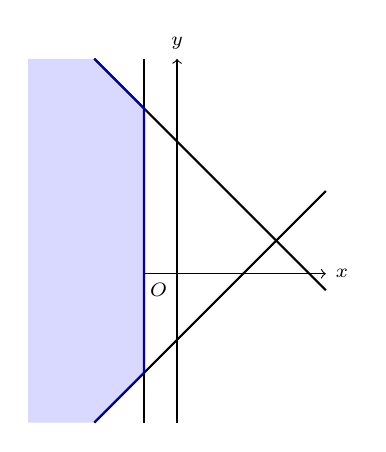
\begin{tikzpicture}[scale=0.42, baseline={(0,1)}]
            \draw[->] (-4.5,0) -- (4.5,0) node[right] {\scriptsize $x$};
            \draw[->] (0,-4.5) -- (0,6.5) node[above] {\scriptsize $y$};
            \fill[blue!15] (-4.5,-4.5) -- (-2.5,-4.5) -- (-1,-3) -- (-1,5) -- (-2.5,6.5) -- (-4.5,6.5) -- cycle;
            \draw[thick] (-2.5,6.5) -- (4.5,-0.5);
            \draw[thick] (-2.5,-4.5) -- (4.5,2.5);
            \draw[thick] (-1,-4.5) -- (-1,6.5);
            \draw[thick, blue!70!black] (-2.5,-4.5) -- (-1,-3) -- (-1,5) -- (-2.5,6.5);
            \node[below left] at (0,0) {\scriptsize $O$};
        \end{tikzpicture}

        \item
        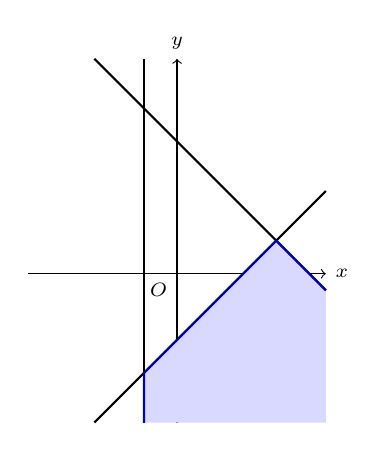
\begin{tikzpicture}[scale=0.42, baseline={(0,1)}]
            \draw[->] (-4.5,0) -- (4.5,0) node[right] {\scriptsize $x$};
            \draw[->] (0,-4.5) -- (0,6.5) node[above] {\scriptsize $y$};
            \fill[blue!15] (-1,-4.5) -- (4.5,-4.5) -- (4.5,-0.5) -- (3,1) -- (-1,-3) -- cycle;
            \draw[thick] (-2.5,6.5) -- (4.5,-0.5);
            \draw[thick] (-2.5,-4.5) -- (4.5,2.5);
            \draw[thick] (-1,-4.5) -- (-1,6.5);
            \draw[thick, blue!70!black] (-1,-4.5) -- (-1,-3) -- (3,1) -- (4.5,-0.5);
            \node[below left] at (0,0) {\scriptsize $O$};
        \end{tikzpicture}

        \item
        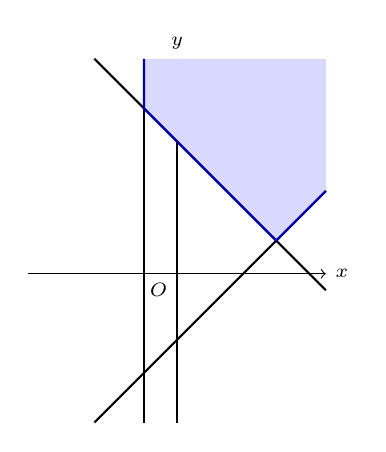
\begin{tikzpicture}[scale=0.42, baseline={(0,1)}]
            \draw[->] (-4.5,0) -- (4.5,0) node[right] {\scriptsize $x$};
            \draw[->] (0,-4.5) -- (0,6.5) node[above] {\scriptsize $y$};
            \fill[blue!15] (-1,6.5) -- (-1,5) -- (3,1) -- (4.5,2.5) -- (4.5,6.5) -- cycle;
            \draw[thick] (-2.5,6.5) -- (4.5,-0.5);
            \draw[thick] (-2.5,-4.5) -- (4.5,2.5);
            \draw[thick] (-1,-4.5) -- (-1,6.5);
            \draw[thick, blue!70!black] (-1,6.5) -- (-1,5) -- (3,1) -- (4.5,2.5);
            \node[below left] at (0,0) {\scriptsize $O$};
        \end{tikzpicture}
    \end{choices}
\end{question}

\begin{solution}
    \textbf{解析：} \\
    本题的关键在于：题目所给的三个不等式并非标准形式，必须先逐一移项整理，才能准确判断每条边界线所对应的取舍方向。 \\[4pt]
    \textbf{整理第一个不等式：} $4 \geq x + y$，将两边对调（不等号方向随之翻转）：
    \[ \displaystyle x + y \leq 4 \]
    表示直线 $x+y=4$ \textbf{下方}（含边界）的区域。 \\[4pt]
    \textbf{整理第二个不等式：} $y - x \geq -2$，移项得：
    \[ \displaystyle y \geq x - 2 \]
    表示直线 $y=x-2$（即 $y-x=-2$）\textbf{上方}（含边界）的区域。 \\[4pt]
    \textbf{整理第三个不等式：} $x + 1 \geq 0$，移项得：
    \[ \displaystyle x \geq -1 \]
    表示直线 $x=-1$ \textbf{右侧}（含边界）的区域。 \\[4pt]
    \textbf{联立三区域：} 三条边界线两两相交，解得三角形顶点：
    \[ \displaystyle x+y=4 \ \cap \ y=x-2 \implies (3,1) \]
    \[ \displaystyle y=x-2 \ \cap \ x=-1 \implies (-1,-3) \]
    \[ \displaystyle x+y=4 \ \cap \ x=-1 \implies (-1,5) \]
    验证原点 $(0,0)$：$0+0=0\leq4$ ✓，$0-0=0\geq-2$ ✓，$0+1=1\geq0$ ✓，
    故原点在区域内，三角形区域应包含原点，与选项 A 的阴影完全吻合。 \\[4pt]
    对于选项 B，其阴影区域位于 $x=-1$ \textbf{左侧}并向左无限延伸，这是把第三个不等式 $x+1\geq0$ 错误地移项为 $x \leq -1$（符号处理错误，忘记不等号在除以正数系数时不需要翻转，却仍然错误地翻转了方向）所致。 \\
    对于选项 C，其阴影区域位于直线 $y=x-2$ \textbf{下方}并向下无限延伸，这是把第二个不等式 $y-x\geq-2$ 误移项为 $y\leq x-2$（移项时符号处理错误）所致。 \\
    对于选项 D，其阴影区域位于直线 $x+y=4$ \textbf{上方}并向上无限延伸，这是把第一个不等式 $4\geq x+y$ 误当作 $x+y\geq4$（对调两边时忘记不等号方向也要随之翻转）所致，这也是本题设计中最容易出错的一步。 \\[4pt]
    综上，唯一正确表示该不等式组解集的图象为选项 A，故选 A。
\end{solution}
%endregion

% 范围：高中数学 - 函数与复合函数 | 考点：换元法求函数解析式（识别已按 g(x) 分解的表达式结构） | 难度：中等
\begin{question}
    已知函数 $g(x) = x + 1$，且$f\big(g(x)\big) = \big(x+1\big)^2 - 3\big(x+1\big) + 5$，求 $f(x)$ 。 \paren[D]
    \begin{choices}
        \item $f(x) = x^2 + 3x + 5$
        \item $f(x) = x^2 - x + 3$
        \item $f(x) = x^2 - 3x + 3$
        \item $f(x) = x^2 - 3x + 5$
    \end{choices}
\end{question}

\begin{solution}
    \textbf{解析：} \\
    本题的关键在于观察到：右边的表达式 $\big(x+1\big)^2 - 3\big(x+1\big) + 5$
    并未展开化简，而是\textbf{完整保留了 $g(x)=x+1$ 这一整体结构}。
    这意味着不必按部就班地令 $t=g(x)=x+1$ 后再反解出 $x=t-1$ 代回原式；
    只需直接把每一处 $x+1$ 看作一个整体符号，替换为 $t$（或直接替换为 $x$）即可。 \\[4pt]
    \textbf{代换：} 设 $t = g(x) = x+1$，则原式变为：
    \[ \displaystyle f(t) = t^2 - 3t + 5 \]
    将 $t$ 换写为 $x$（函数解析式与所用自变量符号无关），得：
    \[ \displaystyle f(x) = x^2 - 3x + 5 \]
    \textbf{验证：} 将 $g(x)=x+1$ 代回验证，
    $f(g(x)) = (x+1)^2 - 3(x+1) + 5$，与题设完全一致，成立。 \\[4pt]
    对于选项 A（$f(x)=x^2+3x+5$），其错误在于换元后的中间项符号处理有误，
    将 $-3t$ 误写成 $+3t$。 \\
    对于选项 B（$f(x)=x^2-x+3$），其错误在于\textbf{没有意识到需要换元}，
    而是直接把已给出的 $f(g(x))$ 表达式完全展开
    （$(x+1)^2-3(x+1)+5 = x^2-x+3$），
    再误把这个关于 $x$ 展开后的式子当作 $f(x)$ 本身——这混淆了"$f$ 复合 $g$ 后关于 $x$ 的表达式"
    与"$f$ 本身的解析式"这两个完全不同的概念。 \\
    对于选项 C（$f(x)=x^2-3x+3$），其错误在于换元后计算常数项时发生了疏漏，
    误将 $t^2-3t+5$ 中的常数项 $5$ 抄写或计算为 $3$。 \\[4pt]
    综上，正确利用"整体代换"思想识别出的解析式为 $f(x) = x^2-3x+5$，故选 D。
\end{solution}

\newpage
%region 范围：函数与图像 | 考点：幂函数、反比例函数图像特征识别（$1/x$、$\sqrt{x}$、$x^2$、$1/x^2$） | 难度：中等
\begin{question}
    观察下列甲、乙、丙、丁四个函数图像，判断下列选项中，函数与图像的配对完全正确的是 \paren[A]

    \begin{center}
    \begin{tabular}{cccc}
    \begin{tikzpicture}[scale=0.55]
        \draw[->] (-2.3,0) -- (2.3,0) node[right] {\scriptsize $x$};
        \draw[->] (0,-2.3) -- (0,2.3) node[above] {\scriptsize $y$};
        \draw[domain=0.3:2.2, samples=40, smooth, thick] plot (\x, {1/\x});
        \draw[domain=-2.2:-0.3, samples=40, smooth, thick] plot (\x, {1/\x});
    \end{tikzpicture}
    &
    \begin{tikzpicture}[scale=0.55]
        \draw[->] (-2.3,0) -- (2.3,0) node[right] {\scriptsize $x$};
        \draw[->] (0,-2.3) -- (0,2.3) node[above] {\scriptsize $y$};
        \draw[domain=0:2, samples=40, smooth, thick] plot (\x, {sqrt(\x)});
    \end{tikzpicture}
    &
    \begin{tikzpicture}[scale=0.55]
        \draw[->] (-2.3,0) -- (2.3,0) node[right] {\scriptsize $x$};
        \draw[->] (0,-2.3) -- (0,2.3) node[above] {\scriptsize $y$};
        \draw[domain=-1.5:1.5, samples=40, smooth, thick] plot (\x, {\x*\x});
    \end{tikzpicture}
    &
    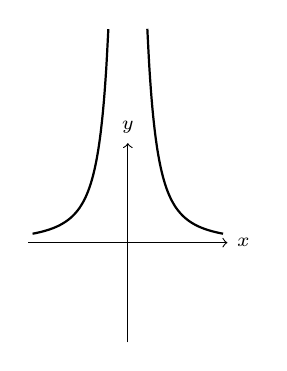
\begin{tikzpicture}[scale=0.55]
        \draw[->] (-2.3,0) -- (2.3,0) node[right] {\scriptsize $x$};
        \draw[->] (0,-2.3) -- (0,2.3) node[above] {\scriptsize $y$};
        \draw[domain=0.45:2.2, samples=40, smooth, thick] plot (\x, {1/(\x*\x)});
        \draw[domain=-2.2:-0.45, samples=40, smooth, thick] plot (\x, {1/(\x*\x)});
    \end{tikzpicture}
    \\
    甲 & 乙 & 丙 & 丁
    \end{tabular}
    \end{center}

    \begin{choices}
        \item 甲：$\displaystyle y=\frac{1}{x}$；乙：$y=\sqrt{x}$；丙：$y=x^2$；丁：$\displaystyle y=\frac{1}{x^2}$
        \item 甲：$\displaystyle y=\frac{1}{x^2}$；乙：$y=\sqrt{x}$；丙：$y=x^2$；丁：$\displaystyle y=\frac{1}{x}$
        \item 甲：$\displaystyle y=\frac{1}{x}$；乙：$y=x^2$；丙：$y=\sqrt{x}$；丁：$\displaystyle y=\frac{1}{x^2}$
        \item 甲：$\displaystyle y=\frac{1}{x^2}$；乙：$y=x^2$；丙：$y=\sqrt{x}$；丁：$\displaystyle y=\frac{1}{x}$
    \end{choices}
\end{question}

\begin{solution}
    \textbf{解析：} \\
    逐一分析四个函数的图像特征：\\
    （1）$\displaystyle y=\frac{1}{x}$：定义域为 $x\neq 0$，是奇函数，图像关于原点对称，由两条分居第一、第三象限的双曲线组成，且随 $|x|$ 增大，函数值趋近于 $0$，与 $x$ 轴、$y$ 轴均不相交——对应甲图。\\
    （2）$y=\sqrt{x}$：定义域为 $x\ge 0$，图像只出现在第一象限（含原点），从原点出发单调递增，且增长速度逐渐变缓（凹向下）——对应乙图。\\
    （3）$y=x^2$：定义域为全体实数，是偶函数，图像关于 $y$ 轴对称，呈开口向上的抛物线，顶点在原点——对应丙图。\\
    （4）$\displaystyle y=\frac{1}{x^2}$：定义域为 $x\neq 0$，是偶函数，图像关于 $y$ 轴对称，函数值恒为正，由两条分居第一、第二象限、且都以 $x$ 轴和 $y$ 轴为渐近线的曲线组成——对应丁图。\\
    选项 B 与 D 都将甲、丁互换，误将 $\displaystyle\frac{1}{x}$（关于原点对称、两支分居一三象限）当作 $\displaystyle\frac{1}{x^2}$（关于 $y$ 轴对称、两支都在 $x$ 轴上方）的图像，忽略了两者对称性与所在象限的本质差异，故 B、D 错误。\\
    选项 C 与 D 都将乙、丙互换，误将 $\sqrt{x}$（仅在第一象限、增长趋缓的曲线）当作 $x^2$（开口向上、左右对称的抛物线）的图像，忽略了定义域与凹凸方向的差异，故 C、D 错误。\\
    综上，只有选项 A 中四个函数与图像的配对完全正确。\\
    故选 A。
\end{solution}
%endregion



% 范围：高中数学 - 函数的值域 | 考点：分式函数值域的求法（反解法／排除法） | 难度：基础
\begin{question}
    求函数 $f(x) = \dfrac{1}{x+2}$ 的值域。 \paren[C]
    \begin{choices}
        \item $R_f = \mathbb{R}$
        \item $R_f = \{y \mid y \neq -2\}$
        \item $R_f = \{y \mid y \neq 0\}$
        \item $R_f = (0, +\infty)$
    \end{choices}
\end{question}

\begin{solution}
    \textbf{解析：} \\
    求分式函数的值域，常用\textbf{反解法}：设 $y = f(x)$，将 $x$ 用 $y$ 表示出来，
    再根据 $x$ 有解的条件反推 $y$ 的取值范围。 \\[4pt]
    \textbf{第一步：设并反解。} 设
    \[ \displaystyle y = \frac{1}{x+2} \]
    两边同乘 $(x+2)$（此时需保证 $x+2 \neq 0$，即 $x \neq -2$，这是原函数的定义域限制）：
    \[ \displaystyle y(x+2) = 1 \implies x + 2 = \frac{1}{y} \implies x = \frac{1}{y} - 2 \]
    \textbf{第二步：反推 $y$ 的取值范围。} \\
    上式中出现了 $\dfrac{1}{y}$，要使这一步的反解有意义，必须满足 $y \neq 0$
    （否则 $\dfrac{1}{y}$ 无意义，即不存在这样的 $x$）。 \\
    反之，对任意 $y \neq 0$，都能由 $x = \dfrac{1}{y} - 2$ 找到对应的 $x$
    （且该 $x$ 自动满足 $x \neq -2$，因为若 $x=-2$ 则 $\dfrac{1}{y}=0$，与 $y\neq0$ 矛盾，不会出现）。 \\
    故值域为 $\{y \mid y \neq 0\}$。 \\[4pt]
    对于选项 A（$\mathbb{R}$），其错误在于忽略了分式函数"分子非零则商恒不为零"这一基本事实，
    误以为分式可以取遍所有实数，包括 $y=0$（但 $\dfrac{1}{x+2}=0$ 无解，因为分子恒为 $1 \neq 0$）。 \\
    对于选项 B（$y \neq -2$），其错误在于\textbf{混淆了定义域与值域}：
    $x \neq -2$ 是原函数\textbf{定义域}的限制条件（分母不为零），
    而非值域的限制条件，属于张冠李戴。 \\
    对于选项 D（$(0,+\infty)$），其错误在于只考虑了 $x > -2$ 时函数取正值的情形，
    而遗漏了 $x < -2$ 时 $x+2 < 0$、函数取负值的情形（例如当 $x=-3$ 时，
    $f(-3) = \dfrac{1}{-1} = -1 < 0$），因而错误地认为值域只能是正数。 \\[4pt]
    综上，函数 $f(x)=\dfrac{1}{x+2}$ 的值域为 $\{y \mid y \neq 0\}$，故选 C。
\end{solution}



% 范围：高中数学 - 角度与弧度、扇形的弧长与面积公式 | 考点：扇形周长与面积的综合应用 | 难度：中等
\begin{question}
    用一根长度为 $100\text{cm}$ 的铁丝弯折成一个半径为 $35\text{cm}$ 的扇形。求该扇形的面积。

    \begin{center}
    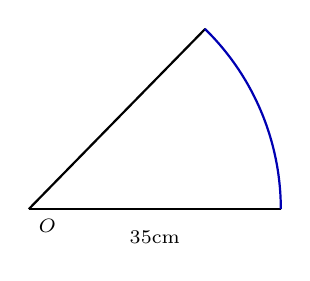
\begin{tikzpicture}[scale=1.6]
        \coordinate (O) at (0,0);
        \coordinate (A) at (2,0);
        \coordinate (B) at (1.4,1.43);
        \draw[thick] (O) -- (A);
        \draw[thick] (O) -- (B);
        \draw[thick, blue!70!black] (A) arc (0:45.7:2);
        \node[below right, font=\scriptsize] at (O) {$O$};
        \node[below, font=\scriptsize] at (1,-0.1) {$35\text{cm}$};
        % \node[above, font=\scriptsize] at (1,1.15) {$35\text{cm}$};
    \end{tikzpicture}
    \end{center}
    \paren[C]
    \begin{choices}
        \item $525\text{cm}^2$
        \item $1050\text{cm}^2$
        \item $1137.5\text{cm}^2$
        \item $1750\text{cm}^2$
    \end{choices}
\end{question}

\begin{solution}
    \textbf{解析：} \\
    本题的关键在于正确区分：铁丝围成的\textbf{周长}包含\textbf{两条半径}与\textbf{一段弧长}，
    而非仅仅是弧长本身，这一点是本题最容易出错之处。 \\[4pt]
    \textbf{第一步：设弧长并列出周长方程。} \\
    设该扇形的弧长为 $l$，半径为 $r=35\text{cm}$。扇形的周长由两条半径与弧长共同构成：
    \[ \displaystyle 2r + l = 100 \]
    代入 $r=35$：
    \[ \displaystyle 2(35) + l = 100 \implies 70 + l = 100 \implies l = 30 \]
    \textbf{第二步：代入扇形面积公式。} \\
    扇形面积公式为
    \[ \displaystyle S = \frac{1}{2} l r \]
    代入 $l=30$，$r=35$：
    \[ \displaystyle S = \frac{1}{2} \times 30 \times 35 = 525 \]
    \textbf{答：该扇形的面积为 $525\text{cm}^2$。} \\[4pt]
    对于选项 A（$1750\text{cm}^2$），其错误在于把整根铁丝的长度 $100$ 直接当作弧长 $l$ 代入公式，
    完全忽略了两条半径也占用了部分铁丝长度，即误算为 $S=\frac{1}{2}(100)(35)$。 \\
    对于选项 B（$1137.5\text{cm}^2$），其错误在于周长方程中只减去了\textbf{一条}半径而非两条，
    即误列方程为 $r+l=100 \implies l=65$，再代入 $S=\frac{1}{2}(65)(35)$。 \\
    对于选项 D（$1050\text{cm}^2$），其错误在于正确求出了 $l=30$，
    但在代入面积公式时遗漏了公式中的 $\frac{1}{2}$，误算为 $S=lr=30\times35$。 \\[4pt]
    综上，该扇形的正确面积为 $525\text{cm}^2$，故选 C。
\end{solution}

% 范围：高中数学 - 角度与弧度的互化 | 考点：角度制与弧度制的转换公式及常见混淆点 | 难度：基础
\begin{question}
    下列关于角度与弧度互化的说法，正确的是： \paren[B]
    \begin{choices}
        \item $1$ 弧度 $= 180°$
        \item $300° = \dfrac{5\pi}{3}$ 弧度
        \item 把角度化为弧度时，应将角度数乘以 $\dfrac{180}{\pi}$
        \item $-\dfrac{2\pi}{3}$ 弧度 $= -150°$
    \end{choices}
\end{question}

\begin{solution}
    \textbf{解析：} \\
    角度与弧度互化的核心公式为：$\pi$ 弧度 $= 180°$，由此可得
    \[ \displaystyle \text{角度} \to \text{弧度：乘以} \ \frac{\pi}{180}, \qquad \text{弧度} \to \text{角度：乘以} \ \frac{180}{\pi} \]
    \textbf{逐项检验：} \\[4pt]
    \textbf{选项 A：} $1$ 弧度并不等于 $180°$，而是等于 $\dfrac{180°}{\pi} \approx 57.3°$。
    该选项的错误在于混淆了"$1$ 弧度"与"$\pi$ 弧度"——只有 $\pi$ 弧度才等于 $180°$，
    误把两者画上了等号。 \\[4pt]
    \textbf{选项 B：} 将 $300°$ 化为弧度，代入公式：
    \[ \displaystyle 300° \times \frac{\pi}{180} = \frac{300\pi}{180} = \frac{5\pi}{3} \]
    与选项所述完全吻合，成立。 \\[4pt]
    \textbf{选项 C：} 该说法把转换方向弄反了——乘以 $\dfrac{180}{\pi}$
    对应的是\textbf{弧度化角度}，而"角度化弧度"应当乘以 $\dfrac{\pi}{180}$，
    此选项恰好把两个转换方向的乘数互换，属于典型的方向混淆错误。 \\[4pt]
    \textbf{选项 D：} 将 $-\dfrac{2\pi}{3}$ 弧度化为角度，代入公式：
    \[ \displaystyle -\frac{2\pi}{3} \times \frac{180}{\pi} = -\frac{2}{3} \times 180° = -120° \]
    而非选项所述的 $-150°$，故该选项在计算过程中出现了数值错误
    （可能是把 $\dfrac{2}{3}$ 误算成 $\dfrac{5}{6}$ 所致）。 \\[4pt]
    综上，唯一正确的说法是选项 B：$300° = \dfrac{5\pi}{3}$ 弧度，故选 B。
\end{solution}


% 范围：高中数学 - 弧度制下扇形的弧长与面积公式 | 考点：由弧度与弧长求扇形面积（公式 $l=r\theta$，$S=\frac{1}{2}lr$） | 难度：中等

\begin{question}
    已知一扇形的圆心角为 $\dfrac{2\pi}{3}$ 弧度，弧长为 $4\pi\text{cm}$，求该扇形的面积。

    \begin{center}
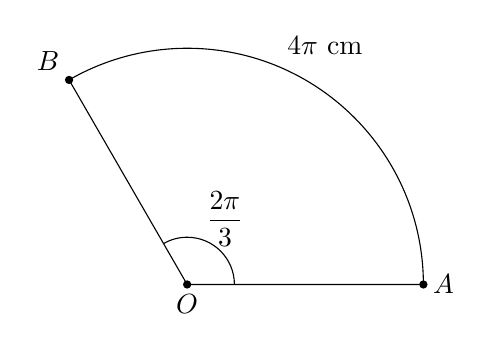
\begin{tikzpicture}[scale=1]\coordinate (O) at (0,0);\coordinate (A) at (3,0);\coordinate (B) at (120:3);\draw (O) -- (A) arc (0:120:3) -- cycle;\fill (O) circle (1.5pt) node[below] {$O$};\fill (A) circle (1.5pt) node[right] {$A$};\fill (B) circle (1.5pt) node[above left] {$B$};\pic[draw,"$\dfrac{2\pi}{3}$",angle radius=6mm,angle eccentricity=1.6]{angle=A--O--B};\node at (60:3.5) {$4\pi\text{ cm}$};\end{tikzpicture}
    \end{center}
    \paren[C]
    \begin{choices}
        \item $24\pi \ \text{cm}^2$
        \item $\dfrac{\pi}{3} \ \text{cm}^2$
        \item $12\pi \ \text{cm}^2$
        \item $\dfrac{4\pi^2}{3} \ \text{cm}^2$
    \end{choices}
\end{question}

\begin{solution}
    \textbf{解析：} \\
    本题需先由弧长公式 $l = r\theta$ 求出半径 $r$，再代入扇形面积公式 $S=\dfrac{1}{2}lr$，
    两步缺一不可，不能直接把弧长与圆心角相乘当作面积。 \\[4pt]
    \textbf{第一步：由 $l=r\theta$ 求半径 $r$。} \\
    已知 $l=4\pi$，$\theta=\dfrac{2\pi}{3}$，代入公式并整理：
    \[ \displaystyle r = \frac{l}{\theta} = \frac{4\pi}{\frac{2\pi}{3}} = 4\pi \times \frac{3}{2\pi} = 6 \]
    \textbf{第二步：代入扇形面积公式 $S=\dfrac{1}{2}lr$。} \\
    \[ \displaystyle S = \frac{1}{2} \times 4\pi \times 6 = 12\pi \]
    \textbf{答：该扇形的面积为 $12\pi \ \text{cm}^2$。} \\[4pt]
    对于选项 A（$24\pi \ \text{cm}^2$），其错误在于正确求出 $r=6$ 后，
    代入面积公式时遗漏了 $\dfrac{1}{2}$，误算为 $S=lr=4\pi\times6$。 \\
    对于选项 B（$\dfrac{\pi}{3} \ \text{cm}^2$），其错误在于求半径时把公式
    $r=\dfrac{l}{\theta}$ 颠倒为 $r=\dfrac{\theta}{l}$，
    算出错误的"半径" $r=\dfrac{2\pi/3}{4\pi}=\dfrac{1}{6}$，再代入面积公式得到此结果。 \\
    对于选项 D（$\dfrac{4\pi^2}{3} \ \text{cm}^2$），其错误在于混淆了面积公式，
    误用 $S=\dfrac{1}{2}l\theta$（把公式中的 $r$ 错当成 $\theta$ 直接代入），
    而没有先求出真正的半径 $r$。 \\[4pt]
    综上，该扇形的正确面积为 $12\pi \ \text{cm}^2$，故选 C。
\end{solution}



\vfill % 与上方内容保持距离

\noindent
\newlength{\sigwidth}
\settowidth{\sigwidth}{（\hspace{4em}师）}

\begin{tabular*}{\textwidth}{@{\extracolsep{\fill}} l l l}
    出题： & 审题： & 审核： \\[4em]
    \rule{\sigwidth}{0.5pt} &
    \rule{\sigwidth}{0.5pt} &
    \rule{\sigwidth}{0.5pt} \\
    （\hspace{0em} \setterteacher ） &
    （\hspace{0em} \reviewteacher ） &
    （\hspace{0em} \auditteacher ） \\
\end{tabular*}


\newpage
\begin{center}
\textbf{参考答案}

\begin{tikzpicture}
  \pgfmathtruncatemacro{\cols}{ifthenelse(\answerkeytotal<=16,8,10)}
  \pgfmathsetlengthmacro{\boxw}{(\linewidth-0.4pt)/\cols}
  \pgfmathsetlengthmacro{\boxh}{1.2cm}
  \pgfmathsetlengthmacro{\offset}{0.15cm}

  \answerkeyitems
\end{tikzpicture}
\end{center}
\end{document}